\documentclass[tikz,border=2pt]{standalone}
\usepackage[T1]{fontenc}
\usepackage{lmodern}
\usepackage{xcolor}
\usetikzlibrary{arrows.meta,calc,positioning}

\definecolor{paletteGreen}{HTML}{2A6F62}
\definecolor{paletteOrange}{HTML}{D96C3D}

\begin{document}
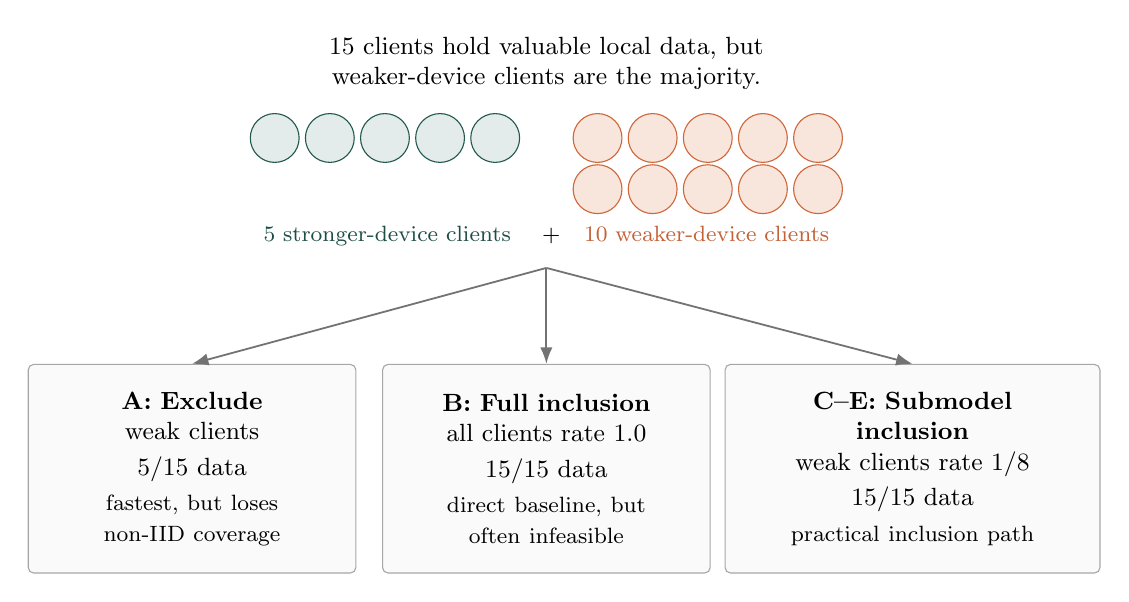
\begin{tikzpicture}[
  labstrong/.style={circle, draw=paletteGreen!80!black, fill=paletteGreen!13, minimum size=6.2mm, inner sep=0pt},
  labweak/.style={circle, draw=paletteOrange!95!black, fill=paletteOrange!18, minimum size=6.2mm, inner sep=0pt},
  decision/.style={rounded corners=2pt, draw=black!35, fill=gray!4, align=center, text width=3.95cm, minimum height=2.65cm, inner sep=3pt, font=\small},
  arrow/.style={-Latex, line width=0.65pt, draw=black!55},
]
\node[align=center, font=\small, text width=7.4cm] at (0, 2.15) {\(15\) clients hold valuable local data, but weaker-device clients are the majority.};

\foreach \x/\y in {-3.45/1.2,-2.75/1.20,-2.05/1.20,-1.35/1.20,-0.65/1.20} {
  \node[labstrong] at (\x,\y) {};
}
\foreach \x/\y in {0.65/1.20,1.35/1.20,2.05/1.20,2.75/1.20,3.45/1.20,0.65/0.55,1.35/0.55,2.05/0.55,2.75/0.55,3.45/0.55} {
  \node[labweak] at (\x,\y) {};
}
\node[font=\footnotesize, align=center] at (0,-0.05) {\textcolor{paletteGreen!70!black}{\(5\) stronger-device clients} \quad+\quad \textcolor{paletteOrange!90!black}{\(10\) weaker-device clients}};

\coordinate (split) at (0,-0.45);
\node[decision] (exclude) at (-4.5,-3) {\textbf{A: Exclude}\\weak clients\\[0.2em]\(5/15\) data\\[0.2em]\footnotesize fastest, but loses non-IID coverage};
\node[decision] (full) at (0,-3) {\textbf{B: Full inclusion}\\all clients rate \(1.0\)\\[0.2em]\(15/15\) data\\[0.2em]\footnotesize direct baseline, but often infeasible};
\node[decision, text width=4.55cm] (submodel) at (4.65,-3) {\textbf{C--E: Submodel}\\\textbf{inclusion}\\weak clients rate \(1/8\)\\[0.2em]\(15/15\) data\\[0.2em]\footnotesize practical inclusion path};

\draw[arrow] (split) -- (exclude.north);
\draw[arrow] (split) -- (full.north);
\draw[arrow] (split) -- (submodel.north);
\end{tikzpicture}
\end{document}
